%% ----------------------------------------------------------------
%% Thesis.tex -- MAIN FILE (the one that you compile with LaTeX)
%% ---------------------------------------------------------------- 

% Set up the document
\documentclass[a4paper, 11pt, oneside]{uet_thesis}  % Use the "Thesis" style, based on the ECS Thesis style by Steve Gunn
\graphicspath{{Figures/}}  % Location of the graphics files (set up for graphics to be in PDF format)

% Include any extra LaTeX packages required
\usepackage[square, numbers, comma, sort&compress]{natbib}  % Use the "Natbib" style for the references in the Bibliography
\usepackage{amsmath}
\usepackage{verbatim}  % Needed for the "comment" environment to make LaTeX comments

\usepackage{vector}  % Allows "\bvec{}" and "\buvec{}" for "blackboard" style bold vectors in maths
\usepackage{float}
\usepackage{url}
\usepackage{natbib}


\hypersetup{urlcolor=blue, colorlinks=true}  % Colours hyperlinks in blue, but this can be distracting if there are many links.

% remove the unnecessary spacing before and after the headings/subheadings
\usepackage[compact]{titlesec}
\titlespacing{\section}{0pt}{*0}{*0}
\titlespacing{\subsection}{0pt}{*0}{*0}
\titlespacing{\subsubsection}{0pt}{*0}{*0}

\setlength{\parskip}{6pt}
%\setlength{\parsep}{0pt}
%\setlength{\headsep}{0pt}
%\setlength{\topskip}{0pt}

%% ----------------------------------------------------------------
\begin{document}
	\frontmatter	  % Begin Roman style (i, ii, iii, iv...) page numbering
	
	% Set up the Title Page
	\title  {Complex Engineering Problem}
	\session {2019 -- 2023}
	\advisor {Prof. Khalid Butt}
	\authors {
		Fariaa Faheem ~~ 2019-EE-1\\
		Marwa Waseem  ~~ 2019-EE-7\\
		Hamza Akhtar  ~~ 2019-EE-12\\
		Filza Shahid  ~~ 2019-EE-151}
	
	\addresses  {\deptname \\ \univname}  % Do not change this here, instead these must be set in the "Thesis.cls" file, please look through it instead
	\date       {\today}
	\subject    {}
	\keywords   {}
	
	\maketitle
	%% ----------------------------------------------------------------
	
	\setstretch{1.3}  % It is better to have smaller font and larger line spacing than the other way round
	
	% Define the page headers using the FancyHdr package and set up for one-sided printing
	\fancyhead{}  % Clears all page headers and footers
	\rhead{\thepage}  % Sets the right side header to show the page number
	\lhead{}  % Clears the left side page header
	
	\pagestyle{fancy}  % Finally, use the "fancy" page style to implement the FancyHdr headers
	
	
	%% Select only one of the certification pages  
	%\CertificationMSc{}
	\CertificationBSc{}
	\clearpage  % Certification ended, now start a new page
	
	
	%% ----------------------------------------------------------------
	% Declaration Page required for the Thesis, your institution may give you a different text to place here
	\Declaration{
		%\addtocontents{toc}{\vspace{1em}}  % Add a gap in the Contents, for aesthetics
		
		I declare that the work contained in this thesis is my own, except where explicitly stated otherwise. In addition this work has not been submitted to obtain another degree or professional qualification.
		
		\bigskip
		
		Signed:~~ \rule[0em]{10em}{1.0pt} \\ % This prints a line for the signature 
		Date:~~~~ \rule[0em]{10em}{1.0pt}  % This prints a line to write the date
	}
	\clearpage     % Declaration ended, now start a new page
	
	%% ----------------------------------------------------------------
	
	\setstretch{1.3}  % Reset the line-spacing to 1.3 for body text (if it has changed)
	
	% The Acknowledgements page, for thanking everyone
	\acknowledgements{
		%\addtocontents{toc}{\vspace{1em}}  % Add a gap in the Contents, for aesthetics
		
		
		
	}
	\clearpage  % End of the Acknowledgements
	
	%% ----------------------------------------------------------------
	% End of the pre-able, contents and lists of things
	% Begin the Dedication page
	\setstretch{1.3}  % Return the line spacing back to 1.3
	\pagestyle{empty}  % Page style needs to be empty for this page
	\dedicatory{Dedicated to ....}
	
	
	%% ----------------------------------------------------------------
	\pagestyle{fancy}  %The page style headers have been "empty" all this time, now use the "fancy" headers as defined before to bring them back
	
	%% ----------------------------------------------------------------
	\lhead{\emph{Contents}}  % Set the left side page header to "Contents"
	\tableofcontents  % Write out the Table of Contents
	
	%% ----------------------------------------------------------------
	\lhead{\emph{List of Figures}}  % Set the left side page header to "List if Figures"
	\listoffigures  % Write out the List of Figures
	
	%% ----------------------------------------------------------------
	\lhead{\emph{List of Tables}}  % Set the left side page header to "List of Tables"
	\listoftables  % Write out the List of Tables
	
	%% ----------------------------------------------------------------
	\setstretch{1.5}  % Set the line spacing to 1.5, this makes the following tables easier to read
	
	
	
	%% ----------------------------------------------------------------
	% The Abstract Page
	
	%\clearpage  % Abstract ended, start a new page
	
	%% ----------------------------------------------------------------
	\mainmatter	  % Begin normal, numeric (1,2,3...) page numbering
	\pagestyle{fancy}  % Return the page headers back to the "fancy" style
	\onehalfspacing
	% Include the chapters of the thesis, as separate files
	% Just uncomment the lines as you write the chapters
	
	% Chapter 1

\chapter{Problem Statement} % Write in your own chapter title
\label{Chapter1}
\lhead{Chapter 1. \emph{Problem Statement}} 
The main objectives of this Complex Engineering Problem are:
\begin{itemize}
	\item To develop programs that store and manage the given data by using four different data structures, that are:
		\begin{enumerate}
			\item Hash Table (Quadratic Probing)
			\item Array
			\item Linked List
			\item Binary Tree
		\end{enumerate}
	\item Implement the following operations on the given data:
		\begin{enumerate}
			\item Insert all of the given data in a data structure.
			\item Print data of data structure in sorted order (traverse in sorted order) (numerically or alphabetically).
			\item Find records.
			\item Delete half of the data from the data structure.			
		\end{enumerate}
	\item To measure execution time and memory consumption for each operation.
	\item To compare operations on different data structures depending on their execution time and memory consumption and conclude which data structure is the best for each operation.
\end{itemize}


 % Introduction 
	
	% Chapter 1

\chapter{File Input} % Write in your own chapter title
\label{Chapter2}
\lhead{Chapter 2. \emph{File Input}} 
 % What to Write 
	
	\chapter{Hash Table Implementation} % Write in your own chapter title
\label{Chapter3}
\lhead{Chapter 3. \emph{Hash Table Implementation}}

\section{Methodology}
Quadratic Probing for Hash tables is used to carryout basic operations on the data array. These basic operations and their working are as follows:

\subsection{Insertion}
First of all, a hash table of size 1.5 times the size of data is created and then the data from the array is inserted into hash table by computing hash function which is id \% table size. On collision the second hash function is calculated and the data is inserted at the appropriate position.

Time Complexity: \textbf{O(1) approaches to O(N)} \\
Space Complexity: \textbf{O(N)}

\subsection{Finding}
In order to find the data, hash function is calculated using the given id. If the required key is found the index of the cell is returned, else by using the formula of quadratic probing the next is cell checked and so on until an empty cell or the required key is reached.

Time Complexity: \textbf{O(N)} \\
Space Complexity: \textbf{O(N)}

\subsection{Sorted Traversal}
For sorted traversal 101, all the IDs of hash table are copied in an array, the array is sorted using quick sort algorithm. The sorted array is traversed, and for the given ID, its location is found in hash table and the data is printed

Sorting Algorithm Used: \textbf{Quick Sort O(log N)} \\
Time Complexity: \textbf{O(N log N)}\\ 
Space Complexity: \textbf{O(N)} \\

For simple sorted traversal, hash table is traversed, the minimum element is found and marked as found, and printed then the other minimum is found and printed and so on.
 Time Complexity: \textbf{O($N^2$)}\\ 
 Space Complexity: \textbf{O(N)} \\ 
\textit{Note: Sorted traversal time complexity is dependent upon sorting algorithm used.}\\
\subsection{Deletion}
Deletion is carried out by finding the cell in which the id to be deleted is present, then the cell is marked as deleted. 

Time Complexity: \textbf{O(1)} \\
Space Complexity: \textbf{O(N)}


\section{Execution Times and Memory Consumptions}
\begin{figure}[H]
	\centering
	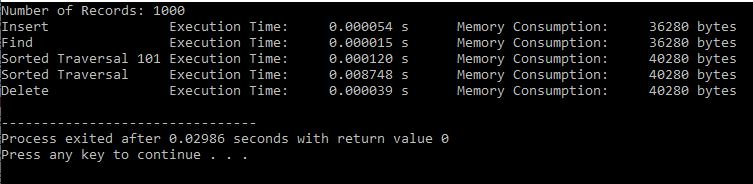
\includegraphics[scale =0.7]{./Figures/hash1000.jpg}
	\rule{35em}{0.5pt}
	\caption{Results for hash implementation with data size 1000.}
	\label{fig:Hash 1000}
\end{figure}

\begin{figure}[H]
	\centering
	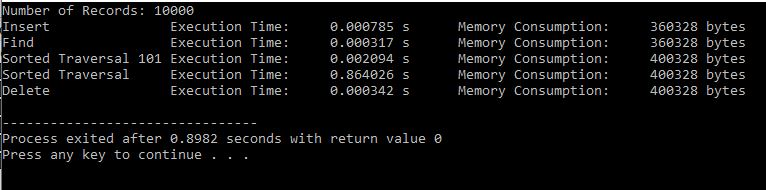
\includegraphics[scale =0.7]{./Figures/hash10000.jpg}
	\rule{35em}{0.5pt}
	\caption{Results for hash implementation with data size 10000.}
	\label{fig:Hash 10000}
\end{figure}

\begin{figure}[H]
	\centering
	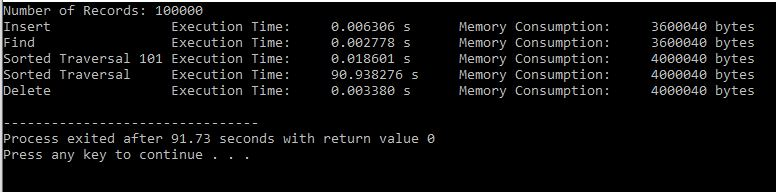
\includegraphics[scale =0.7]{./Figures/hash100000.jpg}
	\rule{35em}{0.5pt}
	\caption{Results for hash implementation with data size 100000.}
	\label{fig:Hash 100000}
\end{figure}

\begin{figure}[H]
	\centering
	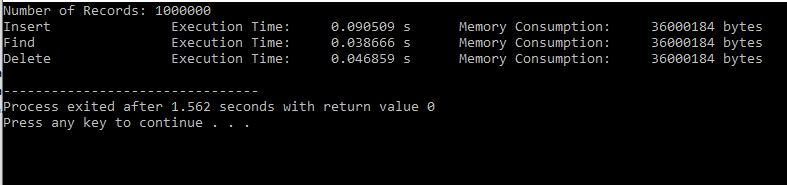
\includegraphics[scale =0.7]{./Figures/hash1000000.jpg}
	\rule{35em}{0.5pt}
	\caption{Results for hash implementation with data size 1000000.}
	\label{fig:Hash 1000000}
\end{figure}
 % Experimental Setup
	
	\chapter{Array Implementation} % Write in your own chapter title
\label{Chapter4}
\lhead{Chapter 4. \emph{Array Implementation}} % Write in your own chapter title to set the page header
\section{Methodology}
Quadratic Probing for Hash tables is used to carryout basic operations on the data array. These basic operations and their working are as follows:

\subsection{Insertion}
First of all an array of size of data is created. The data is inserted at the given index and that cell is marked as legitimate.

Time Complexity: \textbf{O(1)} \\
Space Complexity: \textbf{O(N)}

\subsection{Finding}
In order to find the data, the array is traversed until our required key is found and the index of that cell is returned.

Time Complexity: \textbf{O(N)} \\
Space Complexity: \textbf{O(N)}

\subsection{Sorted Traversal}
For sorted traversal, the array is sorted using quick sort algorithm and then it is traversed to print the data.

Sorting Algorithm Used: \textbf{Quick Sort O(log N)} \\
Time Complexity: \textbf{O(N log N)}\\ 
Space Complexity: \textbf{O(N)} \\

\subsection{Deletion}
Deletion is carried out by finding the cell in which the id to be deleted is present, then the cell is marked as deleted. 

Time Complexity: \textbf{O(1)} \\
Space Complexity: \textbf{O(N)}


\section{Execution Times and Memory Consumptions}
\begin{figure}[H]
	\centering
	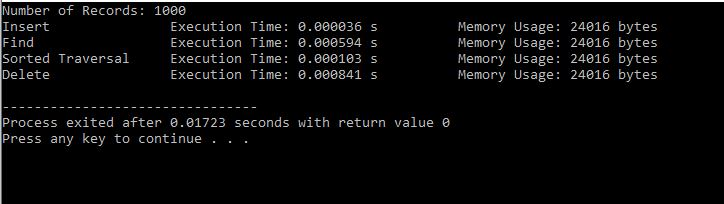
\includegraphics[scale =0.7]{./Figures/Array1000.jpg}
	\rule{35em}{0.5pt}
	\caption{Results for array implementation with data size 1000.}
	\label{fig:Array 1000}
\end{figure}

\begin{figure}[H]
	\centering
	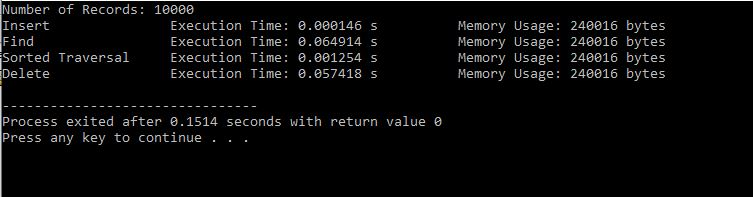
\includegraphics[scale =0.7]{./Figures/Array10000.jpg}
	\rule{35em}{0.5pt}
	\caption{Results for array implementation with data size 10000.}
	\label{fig:Array 10000}
\end{figure}

\begin{figure}[H]
	\centering
	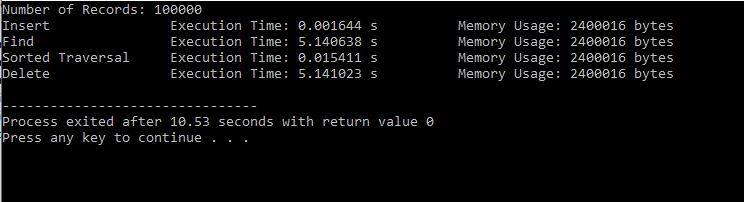
\includegraphics[scale =0.7]{./Figures/Array100000.jpg}
	\rule{35em}{0.5pt}
	\caption{Results for array implementation with data size 100000.}
	\label{fig:Array 100000}
\end{figure}

\begin{figure}[H]
	\centering
	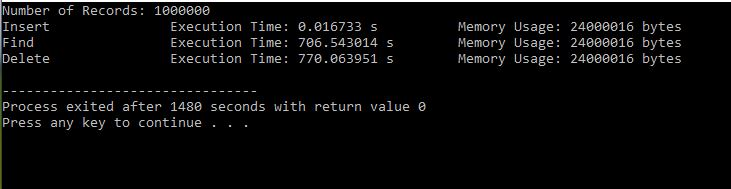
\includegraphics[scale =0.7]{./Figures/Array1000000.jpg}
	\rule{35em}{0.5pt}
	\caption{Results for array implementation with data size 1000000.}
	\label{fig:Array 1000000}
\end{figure}
 % Experiment 1
	
	\chapter{Linked List Implementation} % Write in your own chapter title
\label{Chapter5}
\lhead{Chapter 5. \emph{Linked List Implementation}}
\section{Methodology}
Singley linked lists are used to carryout basic operations on the data array. These basic operations and their working are as follows:

\subsection{Insertion}
Insertion is done by dynamically allocating nodes. Keys i.e., ID's of employees and data is linked with these node. Finally, nodes are inserted at the head of the list.

Time Complexity: \textbf{O(1)} \\
Space Complexity: \textbf{O(N)}

\subsection{Finding}
There is no order in the linked list data like trees so find operation is carried out by simply traversing the list until the required key is found or tail of the list is reached.

Time Complexity: \textbf{O(N)} \\
Space Complexity: \textbf{O(N)}

\subsection{Sorted Traversal}
For sorted traversal, first of all list should be sorted by any convenient sorting algorithm and then traversed from head to tail.

Sorting Algrithm Used: \textbf{Quick Sort O(log N)} \\
Time Complexity: \textbf{O(N log N)}\\ 
Space Complexity: \textbf{O(N)} \\
\textit{Note: Sorted traversal time complexity is dependent upon sorting algorithm used.}\\
\subsection{Deletion}
Deletion is carried out by finding the node to be deleted. This step involves traversing the list. After finding, the node is bypassed by link adjusment and is deleted. 

Time Complexity: \textbf{O(N)} \\
Space Complexity: \textbf{O(N)}

	
\section{Execution Times and Memory Consumptions}
\begin{figure}[H]
	\centering
	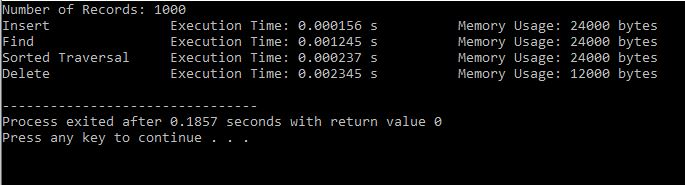
\includegraphics[scale =0.7]{./Figures/List1000.jpg}
	\rule{35em}{0.5pt}
	\caption{Results for linked list implementation with data size 1000.}
	\label{fig:List 1000}
\end{figure}

\begin{figure}[H]
	\centering
	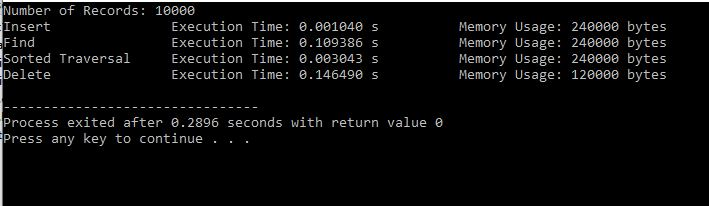
\includegraphics[scale =0.7]{./Figures/List10000.jpg}
	\rule{35em}{0.5pt}
	\caption{Results for linked list implementation with data size 10000.}
	\label{fig:List 10000}
\end{figure}

\begin{figure}[H]
	\centering
	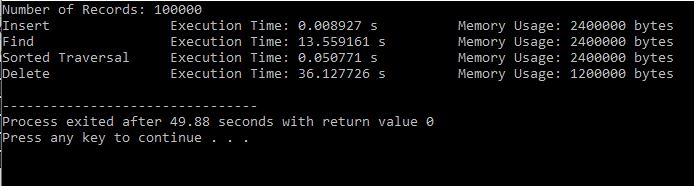
\includegraphics[scale =0.7]{./Figures/List100000.jpg}
	\rule{35em}{0.5pt}
	\caption{Results for linked list implementation with data size 100000.}
	\label{fig:List 100000}
\end{figure} % Experiment 2
	
	\chapter{Tree Implementation} % Write in your own chapter title
\label{Chapter6}
\lhead{Chapter 6. \emph{Tree Implementation}}

\section{Methodology}
Balanced trees are used to carryout basic operation on the data array. These basic operations and their working are as follows:

	\subsection{Insertion}
	Id's of employees are used to populate the self-balancing binary search tree i.e.,\textit{ AVL trees} and then data is linked with the corresponding nodes. Tree is balanced by the phenomenon of left, right, left-right and right-left rotations.
	
	Time Complexity: \textbf{O(log N)} \\
	Space Complexity: \textbf{O(N)}
	
	\subsection{Finding}
	In AVL trees the nodes are arranged in specfic order. Left child node always have key less than the root node and right child will have key greater than the root node. So finding a tree node involves comparing the "key to be found" at each node if its less then only traverse the left subtree and if its larger then traverse the right subtree. In our case we found the even indexed records from data array in tree and measured its execution time and memory consumption.
	
	Time Complexity: \textbf{O(log N)} \\
	Space Complexity: \textbf{O(N)}
	
	\subsection{Sorted Traversal}
	Due to the order propety of AVL trees sorting traversal can be done simply by \textit{inorder traversal} of the tree. In order traversal involves first traversing the left sub-tree recursively then visiting the root node and finally right sub-tree is traversed recursively.
	
	Time Complexity: \textbf{O(N)}   \textit{Note: This time complexity is only for traversal}\\
	Space Complexity: \textbf{O(N)}
	
	\subsection{Deletion}
	Deletion is carried out by going to the tree node to be deleted and then finding the minimum key or element in its right subtree and replacing the node's key with this minimum key. In this way, the order of AVL tree is maintained. In this engineering problem, we deleted all the odd indexed records from the tree.
	
	Time Complexity: \textbf{O(log N)} \\
	Space Complexity: \textbf{O(N)}
	
\section{Execution Times and Memory Consumptions}
\begin{figure}[H].
	\centering
	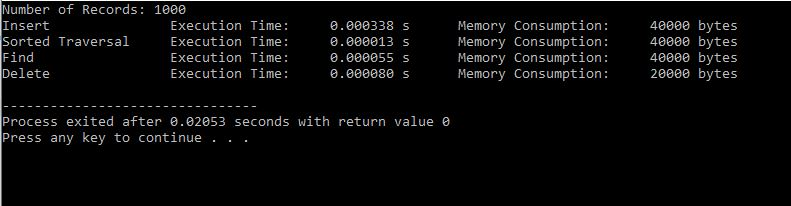
\includegraphics[scale =0.7]{./Figures/Tree1000.jpg}
	\rule{35em}{0.5pt}
	\caption{Results for tree implementation with data size 1000.}
	\label{fig:Tree 1000}
\end{figure}

\begin{figure}[H]
	\centering
	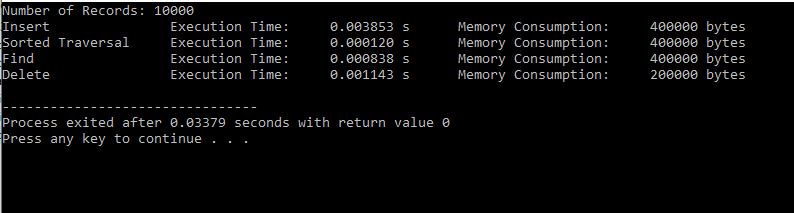
\includegraphics[scale =0.7]{./Figures/Tree10000.jpg}
	\rule{35em}{0.5pt}
	\caption{Results for tree implementation with data size 10000.}
	\label{fig:Tree 10000}
\end{figure}

\begin{figure}[H]
	\centering
	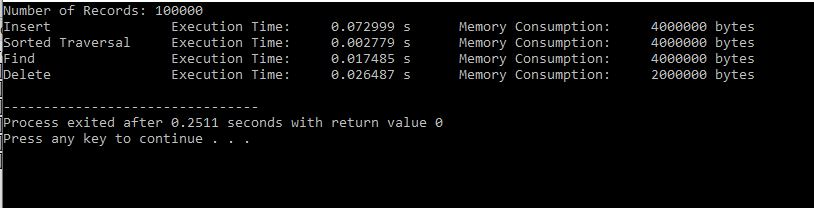
\includegraphics[scale =0.7]{./Figures/Tree100000.jpg}
	\rule{35em}{0.5pt}
	\caption{Results for tree implementation with data size 100000.}
	\label{fig:Tree 100000}
\end{figure}

\begin{figure}[H]
	\centering
	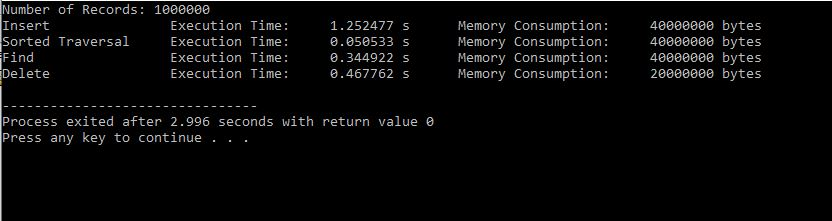
\includegraphics[scale =0.7]{./Figures/Tree1000000.jpg}
	\rule{35em}{0.5pt}
	\caption{Results for tree implementation with data size 1000000.}
	\label{fig:Tree 1000000}
\end{figure}
 %Experiment 3
	
	\chapter{Results} % Write in your own chapter title
\label{Chapter7}
\lhead{Chapter 7. \emph{Results}}

\begin{figure}[H]
	\centering
	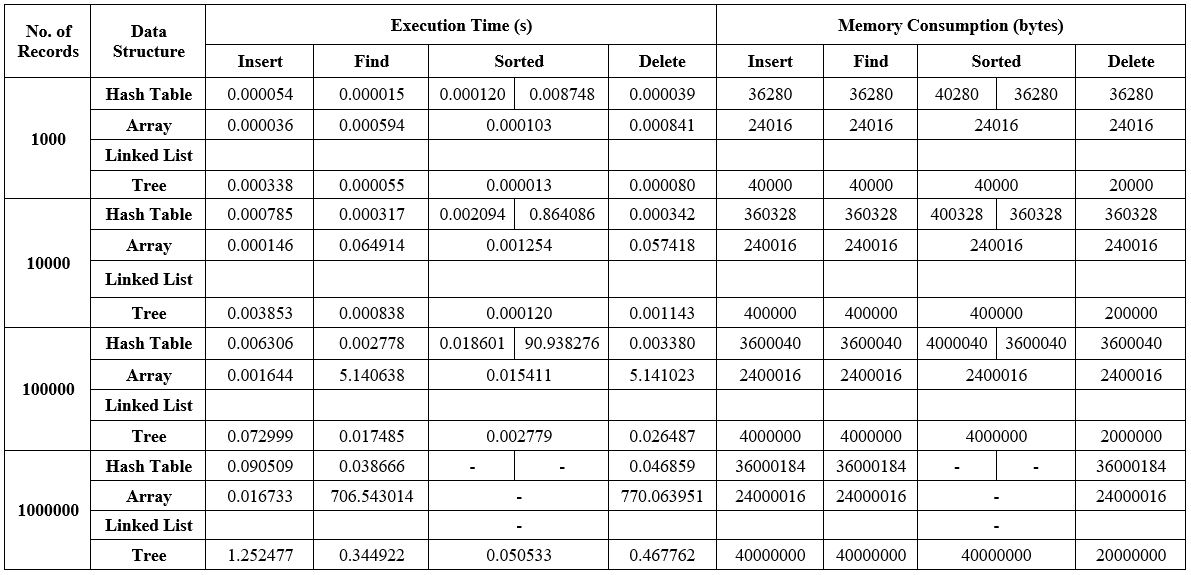
\includegraphics[scale =0.5]{./Figures/result.jpg}
	\rule{35em}{0.5pt}
	\caption{Combined results for all data structures and operations.}
	\label{fig:result}
\end{figure}
 %Experiment 4
	
	%\chapter{Tree Implementation} % Write in your own chapter title
\label{Chapter6}
\lhead{Chapter 6. \emph{Tree Implementation}}

\section{Methodology}
Balanced trees are used to carryout basic operation on the data array. These basic operations and their working are as follows:

	\subsection{Insertion}
	Id's of employees are used to populate the self-balancing binary search tree i.e.,\textit{ AVL trees} and then data is linked with the corresponding nodes. Tree is balanced by the phenomenon of left, right, left-right and right-left rotations.
	
	Time Complexity: \textbf{O(log N)} \\
	Space Complexity: \textbf{O(N)}
	
	\subsection{Finding}
	In AVL trees the nodes are arranged in specfic order. Left child node always have key less than the root node and right child will have key greater than the root node. So finding a tree node involves comparing the "key to be found" at each node if its less then only traverse the left subtree and if its larger then traverse the right subtree. In our case we found the even indexed records from data array in tree and measured its execution time and memory consumption.
	
	Time Complexity: \textbf{O(log N)} \\
	Space Complexity: \textbf{O(N)}
	
	\subsection{Sorted Traversal}
	Due to the order propety of AVL trees sorting traversal can be done simply by \textit{inorder traversal} of the tree. In order traversal involves first traversing the left sub-tree recursively then visiting the root node and finally right sub-tree is traversed recursively.
	
	Time Complexity: \textbf{O(N)}   \textit{Note: This time complexity is only for traversal}\\
	Space Complexity: \textbf{O(N)}
	
	\subsection{Deletion}
	Deletion is carried out by going to the tree node to be deleted and then finding the minimum key or element in its right subtree and replacing the node's key with this minimum key. In this way, the order of AVL tree is maintained. In this engineering problem, we deleted all the odd indexed records from the tree.
	
	Time Complexity: \textbf{O(log N)} \\
	Space Complexity: \textbf{O(N)}
	
\section{Execution Times and Memory Consumptions}
\begin{figure}[H].
	\centering
	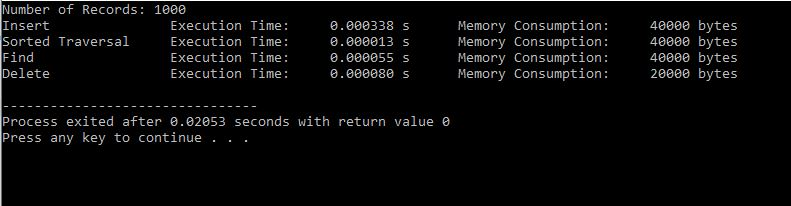
\includegraphics[scale =0.7]{./Figures/Tree1000.jpg}
	\rule{35em}{0.5pt}
	\caption{Results for tree implementation with data size 1000.}
	\label{fig:Tree 1000}
\end{figure}

\begin{figure}[H]
	\centering
	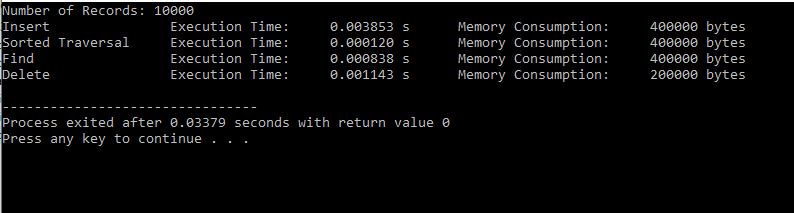
\includegraphics[scale =0.7]{./Figures/Tree10000.jpg}
	\rule{35em}{0.5pt}
	\caption{Results for tree implementation with data size 10000.}
	\label{fig:Tree 10000}
\end{figure}

\begin{figure}[H]
	\centering
	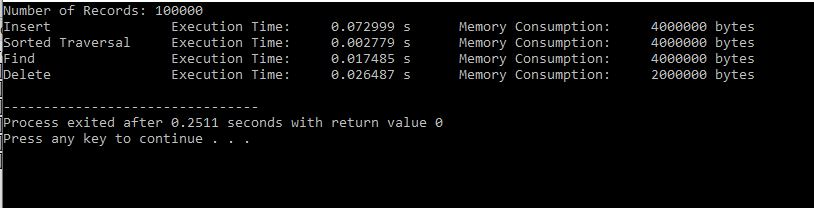
\includegraphics[scale =0.7]{./Figures/Tree100000.jpg}
	\rule{35em}{0.5pt}
	\caption{Results for tree implementation with data size 100000.}
	\label{fig:Tree 100000}
\end{figure}

\begin{figure}[H]
	\centering
	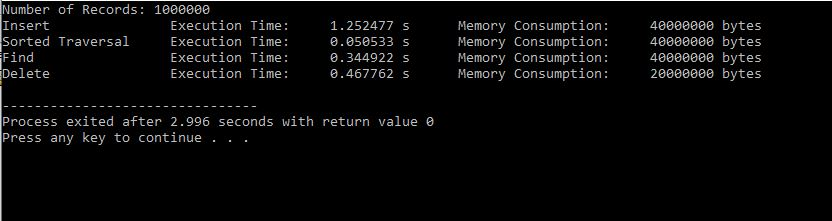
\includegraphics[scale =0.7]{./Figures/Tree1000000.jpg}
	\rule{35em}{0.5pt}
	\caption{Results for tree implementation with data size 1000000.}
	\label{fig:Tree 1000000}
\end{figure}
 % Results and Discussion
	
	%\chapter{Results} % Write in your own chapter title
\label{Chapter7}
\lhead{Chapter 7. \emph{Results}}

\begin{figure}[H]
	\centering
	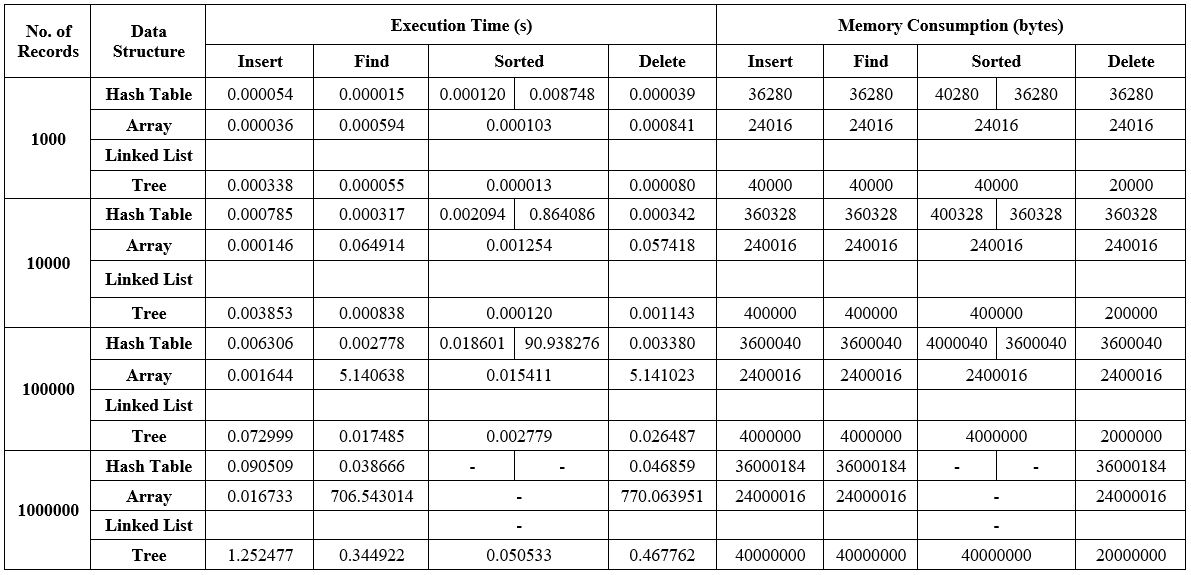
\includegraphics[scale =0.5]{./Figures/result.jpg}
	\rule{35em}{0.5pt}
	\caption{Combined results for all data structures and operations.}
	\label{fig:result}
\end{figure}
 % Conclusion
	
	%% ----------------------------------------------------------------
	% Now begin the Appendices, including them as separate files
	
	%\addtocontents{toc}{\vspace{2em}} % Add a gap in the Contents, for aesthetics
	
	%\appendix % Cue to tell LaTeX that the following 'chapters' are Appendices
	%\input{./Chapters/AppendixA}	% Appendix Title
	
	%\input{./Chapters/AppendixB} % Appendix Title
	
	%\input{./Chapters/AppendixC} % Appendix Title
	
	%\input{./Chapters/AppendixD}
	
	%\addtocontents{toc}{\vspace{2em}}  % Add a gap in the Contents, for aesthetics
	\backmatter
	
	%% ----------------------------------------------------------------
	\begin{thebibliography}{00}
		\bibitem{b1} 
	\end{thebibliography}
	
\end{document}  % The End
%% ----------------------------------------------------------------
